\documentclass{article}

\usepackage{graphicx}
\usepackage{rotating}
\usepackage{amsmath}
\usepackage{mathtools}
\usepackage{nccmath}
\usepackage{tikz}
\usepackage{fancyhdr}
\usepackage{listings}
\usepackage{xcolor}
\usepackage{color}
\usepackage{amsfonts}
\usepackage{textcomp}
\usepackage{float}
\usepackage[sorting=none]{biblatex}
\usepackage[margin=1in]{geometry}
\usepackage[font={small,it}]{caption}
\usepackage{placeins}
\usepackage{xepersian}



%\DeclareMathOperator*{\btie}{\bowtie}
\addbibresource{bibliography.bib}
\settextfont[Scale=1.2]{B-NAZANIN.TTF}
\setlatintextfont[Scale=1]{Times New Roman}
\renewcommand{\baselinestretch}{1.5}
\pagestyle{fancy}
\fancyhf{}
\rhead{تکلیف دوم درس هوش مصنوعی (بخش تئوری)}
\lhead{\thepage}
\rfoot{علیرضا ابره فروش}
\lfoot{9816603}
\renewcommand{\headrulewidth}{1pt}
\renewcommand{\footrulewidth}{1pt}
%%%%%%%%%%
\lstset
{
    language=[latex]tex,
    basicstyle=\ttfamily,
    commentstyle=\color{black},
    columns=fullflexible,
    keepspaces=true,
    upquote=true,
    showstringspaces=false,
    morestring=[s]\\\%,
    stringstyle=\color{black},
}
%%%%%%%%%%
%beginMatlab
\definecolor{mygreen}{RGB}{28,172,0} % color values Red, Green, Blue
\definecolor{mylilas}{RGB}{170,55,241}
%endMatlab
\begin{document}
%beginMatlab
\lstset{language=Matlab,%
    %basicstyle=\color{red},
    breaklines=true,%
    morekeywords={matlab2tikz},
    keywordstyle=\color{blue},%
    morekeywords=[2]{1}, keywordstyle=[2]{\color{black}},
    identifierstyle=\color{black},%
    stringstyle=\color{mylilas},
    commentstyle=\color{mygreen},%
    showstringspaces=false,%without this there will be a symbol in the places where there is a space
    numbers=left,%
    numberstyle={\tiny \color{black}},% size of the numbers
    numbersep=9pt, % this defines how far the numbers are from the text
    emph=[1]{for,end,break},emphstyle=[1]\color{red}, %some words to emphasise
    %emph=[2]{word1,word2}, emphstyle=[2]{style},    
}
%endMatlab
\begin{titlepage}
\begin{center}
\includegraphics[width=0.4\textwidth]{IUT Logo.png}\\
        
\LARGE
\textbf{دانشگاه صنعتی اصفهان}\\
\textbf{دانشکده مهندسی برق و کامپیوتر}\\
        
\vfill
        
\huge
\textbf{عنوان: تکلیف اول درس سیستم‌های عامل 1}\\
        
\vfill
        
\LARGE
\textbf{نام و نام خانوادگی: علیرضا ابره فروش}\\
\textbf{شماره دانشجویی: 9816603}\\
\textbf{نیم\,سال تحصیلی: پاییز 1400}\\
\textbf{مدرّس: دکتر محمّدرضا حیدرپور}\\
\textbf{دستیاران آموزشی: مجید فرهادی - دانیال مهرآیین - محمّد نعیمی}\\
\end{center}
\end{titlepage}


%\tableofcontents
\newpage


\section{نوید زندانی}
\subsection{قیدهای \lr{binary} و \lr{unary}}
\begin{fleqn}
\begin{equation}
\begin{aligned}
\forall i\in \left\{ 1,2,3,4,5,6 \right\}\:\:\:\:\:\: Y_{i} = \begin{cases}
    0 & X_{i} = \text{زندان} \\
    1 & X_{i} = \text{خروج} \\
    2 & X_{i} = \text{چاه}
\end{cases}
\end{aligned}
\end{equation}
\end{fleqn}


\begin{fleqn}
\begin{equation}
\begin{aligned}
C_{1} = \left\langle \left( X_{1},\: X_{2} \right),\: \max\left\{ Y_{1},\: Y_{2} \right\} = 1 \right\rangle \\
C_{2} = \left\langle \left( X_{2},\: X_{3} \right),\: \max\left\{ Y_{2},\: Y_{3} \right\} = 1 \right\rangle \\
C_{3} = \left\langle \left( X_{3},\: X_{4} \right),\: \max\left\{ Y_{3},\: Y_{4} \right\} = 2 \right\rangle \\
C_{4} = \left\langle \left( X_{4},\: X_{5} \right),\: \max\left\{ Y_{4},\: Y_{5} \right\} = 2 \right\rangle \\
C_{5} = \left\langle \left( X_{5},\: X_{6} \right),\: \max\left\{ Y_{5},\: Y_{6} \right\} = 2 \right\rangle \\
C_{6} = \left\langle \left( X_{6},\: X_{1} \right),\: \max\left\{ Y_{6},\: Y_{1} \right\} = 2 \right\rangle
\end{aligned}
\end{equation}

\begin{equation}
\begin{aligned}
C_{7} = \left\langle \left( X_{1},\: X_{2} \right),\: Y_{1} \times Y_{2} \neq 1 \right\rangle \\
C_{8} = \left\langle \left( X_{2},\: X_{3} \right),\: Y_{2} \times Y_{3} \neq 1 \right\rangle \\
C_{9} = \left\langle \left( X_{3},\: X_{4} \right),\: Y_{3} \times Y_{4} \neq 1 \right\rangle \\
C_{10} = \left\langle \left( X_{4},\: X_{5} \right),\: Y_{4} \times Y_{5} \neq 1 \right\rangle \\
C_{11} = \left\langle \left( X_{5},\: X_{6} \right),\: Y_{5} \times Y_{6} \neq 1 \right\rangle \\
C_{12} = \left\langle \left( X_{6},\: X_{1} \right),\: Y_{6} \times Y_{1} \neq 1 \right\rangle
\end{aligned}
\end{equation}
\end{fleqn}







\subsection{}%2
\subsection{}%3
با توجه به اینکه دامنه‌های متغیرهای \lr{$X_{4}$} و \lr{$X_{6}$} تک عضوی است و سایر متغیرها دامنه‌های بیش از یک عضوی دارند، طبق \lr{MRV} متغیرهای \lr{$X_{4}$} و \lr{$X_{6}$} پیش از بقیه مقداردهی می‌شوند.
\subsection{}%4
در این صورت داریم: \\
\begin{fleqn}
\begin{equation}
\begin{aligned}
X_{5} = \text{زندان} \:\:\:\: \Rightarrow \:\:\:\:
Y_{5} = 0
\end{aligned}
\end{equation}
\end{fleqn}
برای اینکه قیدهای \lr{$C_{4}$} و \lr{$C_{5}$} ارضا شوند، دامنه‌های \lr{$X_{4}$} و \lr{$X_{6}$} برابر $\left\{ چاه \right\}$ می‌شود. با انتخاب مقدار چاه برای دو متغیر، و برای ارضای قیود \lr{$C_{1}$} و \lr{$C_{2}$} و \lr{$C_{7}$} و \lr{$C_{8}$}، دو راه‌حل ممکن زیر برای این مسئله وجود دارد: \\
\begin{fleqn}
\begin{equation}
\begin{aligned}
X = \left( \text{زندان}, \: \text{خروج}, \: \text{زندان}, \: \text{چاه}, \: \text{زندان}, \: \text{چاه} \right) \\
X = \left( \text{خروج}, \: \text{زندان}, \: \text{خروج}, \: \text{چاه}, \: \text{زندان}, \: \text{چاه} \right) \\
\end{aligned}
\end{equation}
\end{fleqn}

\subsection{}%5
\subsection{}%6



\section{مسئله سه رنگ}
از آنجایی که هیچ راسی وجود ندارد که با مقداردهی آن دامنه‌ی راسی دیگر تهی شود پس  \lr{arc-consistency} برقرار است. همچنین از آنجایی که هیچ دو راسی وجود ندارد که با مقداردهی آن‌ها، دامنه‌ی راسی دیگر تهی شود \lr{path-consistency} نیز در این مسئله برقرار است. اما چون اگر سه راس را با سه رنگ متفاوت رنگ کنیم، برای راس چهارم رنگی باقی نمی‌ماند پس \lr{4-consistency} برقرار نمی‌باشد. با اضافه کردن قیود باینری زیر می‌توانیم مسئله را \lr{4-consistent} کنیم ($X_{i}$ها رنگ‌های نظیر راس‌های گراف هستند). \\
\begin{fleqn}
\begin{equation}
\begin{aligned}
C_{1} = \left\langle \left( X_{1},\: X_{2} \right),\: X_{1} \neq X_{2} \right\rangle \\
C_{2} = \left\langle \left( X_{2},\: X_{3} \right),\: X_{2} \neq X_{3} \right\rangle \\
C_{3} = \left\langle \left( X_{3},\: X_{4} \right),\: X_{3} \neq X_{4} \right\rangle \\
C_{4} = \left\langle \left( X_{4},\: X_{1} \right),\: X_{4} \neq X_{1} \right\rangle \\
C_{5} = \left\langle \left( X_{1},\: X_{3} \right),\: X_{1} \neq X_{3} \right\rangle \\
C_{6} = \left\langle \left( X_{4},\: X_{2} \right),\: X_{4} \neq X_{2} \right\rangle
\end{aligned}
\end{equation}
\end{fleqn}



\section{\lr{consistency}}
\subsection{}
خیر. الزامی وجود ندارد. در واقع می‌توان با مقداردهی مناسب، درجات بالای سازگاری را محقق کنیم، درحالی که درجات پایین سازگاری برقرار نباشند. برای مثال در \lr{CSP}ِ $P$ \lr{arc-consistency} برقرار می‌باشد، اما \lr{node-consistency} نداریم. \\
\begin{fleqn}
\begin{equation}
\begin{aligned}
P = (X,\:D,\:C) \\ \\
X = \left\{ X_{1},\:X_{2} \right\} \\
D = \left\{ D_{1},\:D_{2} \right\} \\
C = \left\{ C_{1},\:C_{2} \right\} \\ \\
D_{1} = \left\{ 1,\:2,\:3,\:4 \right\} \\
D_{2} = \left\{ 1,\:2,\:3,\:4 \right\} \\
C = \left\{ C_{1},\:C_{2} \right\}\\
C_{1} = \left\langle \left( X_{1} \right),\: X_{1} \le 3 \right\rangle\\
C_{2} = \left\langle \left( X_{1},\: X_{2} \right),\: X_{1} = X_{2} \right\rangle
\end{aligned}
\end{equation}
\end{fleqn}
\subsection{}

\section{مدل‌سازی}
\subsection{}
جمعیت شهر $i$ را با $X_{i}$ نمایش می‌دهیم. \lr{CSP} به شکل زیر مدل می‌شود.\\
\begin{fleqn}
\begin{equation}
\begin{aligned}
P = (X,\:D,\:C) \\ \\
X = \left\{ X_{1},\:X_{2},\:\cdots ,\:X_{n} \right\} \\
D = \left\{ D_{1},\:D_{2},\:\cdots ,\:D_{n} \right\} \\
C = \left\{ C_{1},\:C_{2},\:\cdots ,\:C_{m+1} \right\} \\ \\
\forall i:\:\:\:\:D_{i} = \mathbb{W} \\
\forall \:\: 1 \le i \leq j \le n \:\: | \:\: i \text{همسایه} j, \:\: \exists k: \:\:\:\:C_{k} = \left\langle \left( X_{i},\:X_{j} \right),\: \left| X_{i} - X_{j} \right| \ge 2000 \right\rangle\\
C_{m+1} = \left\langle \left( X_{\arg\: \max_{i}\left\{ X_{i} \right\}},\:X_{\arg\: \min_{j}\left\{ X_{j} \right\}} \right),\: \max_{i}\left\{ X_{i} \right\} \le 3\min_{j}\left\{ X_{j} \right\} \right\rangle
\end{aligned}
\end{equation}
\end{fleqn}


\subsection{}
فرض می‌کنیم که نقشه‌ی مورد نظر نقشه‌ی استرالیا باشد. رنگ راس‌ها را با \lr{WA}، \lr{NT}، \lr{Q}، \lr{NSW}، \lr{SA}، \lr{V} و \lr{T} نشان می‌دهیم. \lr{CSP} به شکل زیر مدل می‌شود.\\
$
Y_{w} = \text{تعداد رئوس با رنگ سفید} \\
Y_{r} = \text{تعداد رئوس با رنگ قرمز} \\
Y_{g} = \text{تعداد رئوس با رنگ سبز} \\
Y_{b} = \text{تعداد رئوس با رنگ آبی} \\ \\
P = (X,\:D,\:C) \\ \\
X = \left\{ WA,\:NT,\:Q,\:NSW,\:SA,\:V,\:T \right\} \\
D = \left\{ D_{WA},\:D_{NT},\:D_{Q},\:D_{NSW},\:D_{SA},\:D_{V},\:D_{T} \right\} \\
C = \left\{ C_{1},\:C_{2},\:\cdots ,\:C_{9} \right\} \\ \\
D_{WA}=D_{NT}=D_{Q}=D_{NSW}=D_{SA}=D_{V}=D_{T}=\left\{ w,\:r,\:g,\:b \right\} \\
C_{1} = \left\langle \left( SA,\:WA \right),\: SA \neq WA \right\rangle \\
C_{2} = \left\langle \left( SA,\:NT \right),\: SA \neq NT \right\rangle \\
C_{3} = \left\langle \left( SA,\:Q \right),\: SA \neq Q \right\rangle \\
C_{4} = \left\langle \left( SA,\:NSW \right),\: SA \neq NSW \right\rangle \\
C_{5} = \left\langle \left( SA,\:V \right),\: SA \neq V \right\rangle \\
C_{6} = \left\langle \left( NT,\:WA \right),\: NT \neq WA \right\rangle \\
C_{7} = \left\langle \left( Q,\:NT \right),\: Q \neq NT \right\rangle \\
C_{8} = \left\langle \left( NSW,\:Q \right),\: NSW \neq Q \right\rangle \\
C_{9} = \left\langle \left( V,\:NSW \right),\: V \neq NSW \right\rangle \\
C_{10} = \left\langle \left( WA,\:NT,\:Q,\:NSW,\:SA,\:V,\:T \right),\: Y_{w} \le Y_{r} \le Y_{g} \le Y_{b} \right\rangle \\
C_{11} = \left\langle \left( WA,\:NT,\:Q,\:NSW,\:SA,\:V,\:T \right),\: Y_{b} \le 2Y_{w} \right\rangle \\
$






\section{برنامه‌ریزی کلاس‌ها}
\subsection{}
مسئله را به شکل \lr{CSP}ِ زیر مدل می‌کنیم: \\
$
X_{1} = \text{استاد کلاس 1} \\
X_{2} = \text{استاد کلاس 2} \\
X_{3} = \text{استاد کلاس 3} \\
X_{4} = \text{استاد کلاس 4} \\
X_{5} = \text{استاد کلاس 5} \\
\\
D_{1} = \left\{ \text{پ} \right\} \\
D_{2} = \left\{ \text{ب}, \: \text{پ} \right\} \\
D_{3} = \left\{ \text{الف}, \: \text{ب}, \: \text{پ} \right\} \\
D_{4} = \left\{ \text{الف}, \: \text{ب}, \: \text{پ} \right\} \\
D_{5} = \left\{ \text{ب}, \: \text{پ} \right\} \\
\\
C_{1} = \left\langle \left( X_{1},\: X_{2} \right),\: X_{1} \neq X_{2} \right\rangle \\
C_{2} = \left\langle \left( X_{2},\: X_{3} \right),\: X_{2} \neq X_{3} \right\rangle \\
C_{3} = \left\langle \left( X_{3},\: X_{4} \right),\: X_{3} \neq X_{4} \right\rangle \\
C_{4} = \left\langle \left( X_{4},\: X_{2} \right),\: X_{4} \neq X_{2} \right\rangle \\
C_{5} = \left\langle \left( X_{4},\: X_{5} \right),\: X_{4} \neq X_{5} \right\rangle \\
C_{6} = \left\langle \left( X_{5},\: X_{3} \right),\: X_{5} \neq X_{3} \right\rangle \\
\\
\\
X = \left\{ X_{1},\: X_{2},\: X_{3},\: X_{4},\: X_{5} \right\} \\
D = \left\{ D_{1},\: D_{2},\: D_{3},\: D_{4},\: D_{5} \right\} \\
C = \left\{ C_{1},\: C_{2},\: C_{3},\: C_{4},\: C_{5},\: C_{6} \right\} \\
$

\subsection{}
%graph
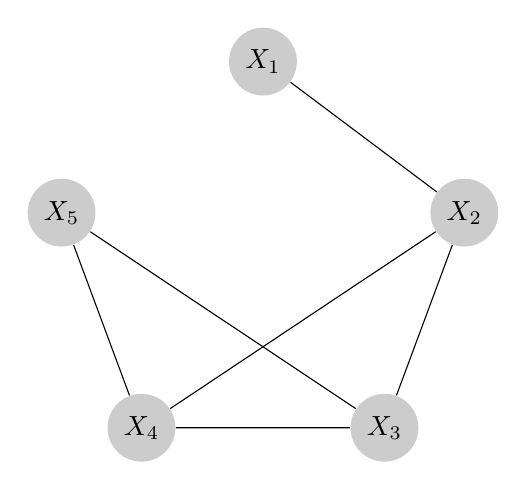
\begin{tikzpicture}
  [scale=.8,auto=left,every node/.style={circle,fill=black!20}]
  \node (n1) at (0,3.3125) {$X_{1}$};
  \node (n2) at (3.197,0.91475)  {$X_{2}$};
  \node (n3) at (1.9285,-2.5)  {$X_{3}$};
  \node (n4) at (-1.9285,-2.5) {$X_{4}$};
  \node (n5) at (-3.197,0.91475)  {$X_{5}$};

  \foreach \from/\to in {n1/n2,n2/n3,n2/n4,n3/n4,n3/n5,n4/n5}
    \draw (\from) -- (\to);

\end{tikzpicture}
%graph

\subsection{}
ثابت می‌شود که هر \lr{CSP}ای که ساختار درخت‌گونه داشته باشد را می‌توان در زمان چندجمله‌ای حل کرد. پس ترجيح مي‌دهيم مسائل \lr{CSP} با ساختار درخت را حل كنيم.

\section{\lr{Puzzle Cryptarithmetic}}
در ابتدا اندازه‌ی همه دامنه‌ها با یکدیگر برابراند (ارقام صفر تا 9). طبق فرض دامنه‌ی $M$ و $S$ صفر ندارند. همچنین از آنجایی که جمع دو عدد 4 رقمی ماکسیمم 19998 است، پس بیشترین مقداری که $M$ می‌تواند بگیرد مقدار 1 است. در نتیجه دامنه‌ی $M$ به مجموعه‌ی تک‌عضوی 1 اصلاح می‌شود. طبق \lr{MRV} متغیر $M$ را مقداردهی می‌کنیم. تنها مقدار دامنه‌ی $M$ یعنی 1 را انتخاب می‌کنیم. با توجه به قید \lr{Alldiff}، عضو 1 از دامنه‌ی سایر متغیرها حذف می‌شود.\\
در جمع ارقام ‌هزارگان (ارقام $S$ و $M$)، چون \lr{Carry} یک داریم، پس 
$S+1 \ge 9$.
دامنه‌ی متغیر $S$ مجموعه‌ی شامل 8 و 9 است. طبق \lr{MRV} متغیر $S$ را مقداردهی می‌کنیم. برای اینکه \lr{Carry}ِ یک داشته باشیم، $S$ تنها در صورتی می‌تواند مقدار 8 را بگیرد که \lr{Carry}ِ یک از قبل داشته باشد. پس طبق \lr{LCV} مقداری را انتخاب می‌کنیم که کمترین محدودیت را در دامنه‌های بقیه‌ی متغیرها ایجاد کند. پس به $S$ مقدار 9 را می‌دهیم. عضو 9 از دامنه‌ی سایر متغیرها حذف می‌شود. توجه شود که اگر در این شاخه به جواب نرسیم باید بازگشت به عقب داشته باشیم و به $S$ مقدار 8 بدهیم.\\
با توجه به اینکه 
$O=S+M-10$،
دامنه‌ی $O$ به مجموعه‌ی تک‌عضوی 0 اصلاح می‌شود. طبق \lr{MRV} متغیر $O$ را مقداردهی می‌کنیم. تنها مقدار دامنه‌ی $O$ یعنی 0 را انتخاب می‌کنیم. عضو 0 از دامنه‌ی سایر متغیرها حذف می‌شود.\\
با توجه به قید \lr{Alldiff} $N=E+1$. و چون \lr{Carry}ِ یک داریم، $E+10= N+R+Carry$. پس 
$R+Carry=9$.
چون دامنه‌ی $R$ مقدار 9 ندارد، پس \lr{Carry} برابر 1 و دامنه‌ی $R$ به مجموعه‌ی تک‌عضوی 8 اصلاح می‌شود. طبق \lr{MRV} متغیر $R$ را مقداردهی می‌کنیم. تنها مقدار دامنه‌ی $R$ یعنی 8 را انتخاب می‌کنیم. عضو 8 از دامنه‌ی سایر متغیرها حذف می‌شود.\\
چون
$N=E+1$
و مقادیر 0، 1، 8 و 9 از دامنه‌ها حذف شده‌اند، دامنه‌های $E$ و $N$ به ترتیب مجموعه‌ی شامل ارقام 2 تا 6 و ارقام 3 تا 7 است. طبق \lr{MRV} یکی از دو متغیر $E$ و $N$ را را باید مقداردهی ‌کنیم. حال طبق \lr{Degree} متغیری که درجه‌ی کمتری در گراف محدودیت دارد را انتخاب می‌کنیم. پس متغیر $N$ انتخاب می‌شود. از آنجایی که از یکان به دهگان \lr{Carry} داریم، 
$D+E \ge 10$
برقرار است و چون
$N=E+1$
هر چه $N$ بزرگ‌تر انتخاب شود، $E$ هم بزرگ‌تر خواهد بود و در نتیجه برای $D$ مقادیر بیشتری از دامنه‌اش را باقی می‌گذارد. پس $N$ را بزرگ‌ترین مقدار دامنه‌اش یعنی 7 مقداردهی می‌کنیم. با فرض اینکه این شاخه به یک جواب منتهی نمی‌شود، بازگشت به عقب رخ می‌دهد و مقدار 6 را به $N$ می‌دهیم. عضو 6 از دامنه‌ی سایر متغیرها حذف می‌شود.\\
حال چون 
$N=E+1$
$E$ را با 5 مقداردهی می‌کنیم. عضو 5 از دامنه‌ی سایر متغیرها حذف می‌شود.\\
چون از یکان به دهگان \lr{Carry} داشتیم، پس 
$D+5 \ge 10$
پس 
$D \ge 5$
چون از بین ارقام 5 تا 9 تنها 7 در دامنه‌ی \lr{D} باقی‌مانده است، آن را با 7 مقدارهی می‌کنیم. در نهایت برای متغیر $Y$ مقدار 2 به دست می‌آید. درخت در شروع به شکل زیر است.
%graph
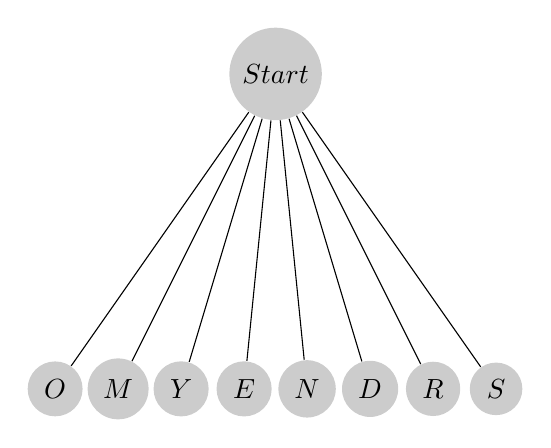
\begin{tikzpicture}
  [scale=.8,auto=left,every node/.style={circle,fill=black!20}]
  \node (n1) at (0.5,5)  {$Start$};
  \node (n2) at (-3,0)  {$O$};
  \node (n3) at (-2,0)  {$M$};
  \node (n4) at (-1,0)  {$Y$};
  \node (n5) at (0,0)  {$E$};
  \node (n6) at (1,0)  {$N$};
  \node (n7) at (2,0)  {$D$};
  \node (n8) at (3,0)  {$R$};
  \node (n9) at (4,0)  {$S$};

  \foreach \from/\to in {n1/n2,n1/n3,n1/n4,n1/n5,n1/n6,n1/n7,n1/n8,n1/n9}
    \draw (\from) -- (\to);

\end{tikzpicture}
%graph
%%%%%%%%%%%%%%%%%%%%%%%%%%%%%%%%%%%
%%%%%%%%%%%%%%%%%%%%%%%%%%%%%%%%%%%
%%%%%%%%%%%%%%%%%%%%%%%%%%%%%%%%%%%

\section*{منابع}
\renewcommand{\section}[2]{}%
\begin{thebibliography}{99} % assumes less than 100 references
%چنانچه مرجع فارسی نیز داشته باشید باید دستور فوق را فعال کنید و مراجع فارسی خود را بعد از این دستور وارد کنید


\begin{LTRitems}

\resetlatinfont

\bibitem{b1}
\end{LTRitems}

\end{thebibliography}


\end{document}
